\documentclass{article}
\usepackage[utf8]{inputenc}
\usepackage{fancyhdr}
\usepackage[left=2cm, right=2cm, top=2cm, bottom=2cm]{geometry}
\usepackage{parskip}
\usepackage{algpseudocode}
\usepackage{color}
\usepackage{wrapfig}
\usepackage{graphicx}
\usepackage{amsmath}
\usepackage{amssymb}

\pagestyle{fancy}

\begin{document}

\lhead{LINMA2710 - Project 2}
\rhead{Adrien Banse (12501700)}
\cfoot{}

\section{Problem considered}
\label{problem}
For  some function $u: \Omega \to \mathbb{R}$, consider the following diffusion problem:
\begin{equation}
\label{PDE}
\begin{aligned}
	\frac{\partial u(t, x, y)}{\partial t} = \alpha \left( \frac{\partial^2 u(t, x, y)}{\partial x^2} + \frac{\partial^2 u(t, x, y)}{\partial y^2} \right), \\
	u(0, x, y) = u_0(x, y).
\end{aligned}
\end{equation}
Equation~\eqref{PDE} is a special case of the diffusion problem considered in the statement, with $D(x, y) = \alpha$ and $f(x, y) = 0$ for all $x, y$. We consider the following values for the problem: 
\begin{itemize}
	\item $\Omega = [0, 300] \times [0, 50] \times [0, 50]$,
	\item $\alpha = 2$, 
	\item $u_0: [0, 50] \times [0, 50] \to \mathbb{R}$ defined as: for all $y \in [0, 50]$ $u_0(0, y) = 100$ and for all $(x, y) \in (0, 50] \times [0, 50]$, $u_0(x, y) = 0$.
\end{itemize}
Note that a physical way to interpret Equation~\eqref{PDE} is to consider the diffusion of \emph{heat} on a 2D plate of dimensions 50[m] $\times$ 50[m] during 300[s], from an intial state. $u(t, x, y)$ is thus the temperature in [K] at time $t$[s] at the point at $x$[m] of the origin of the plate in one direction and $y$[m] of the origin in the other direction\footnote{[m] stands for \emph{meters}, [s] for \emph{seconds} and [K] for \emph{Kelvin}.}. The intial state is when only the upper part of the plate has temperature $100$[K].

Consider that, with the same notations as in the statement, we choose somes values of $\Delta t$, $\Delta x$, $\Delta y$, then the explicit scheme is numerically stable if \cite[Equations (3.5), (3.6)]{morton_mayers_2005}:
\begin{equation}
\label{stable}
	\frac{\alpha \Delta t}{\Delta x^2} + \frac{\alpha \Delta t}{\Delta y^2} \leq \frac{1}{2} \iff \Delta t \leq \frac{1}{2\alpha} \frac{\Delta x^2 \Delta y^2}{\Delta x^2 + \Delta y^2}.
\end{equation}

\section{Results}
Following condition~\eqref{stable}, we choose to numerically solve~\eqref{PDE} (still with the same notations as in the statement): 
\begin{itemize}
	\item $\Delta x = \Delta y = 1$, thus $n_x = n_y = 50$,
	\item according to Equation~\ref{stable}, $\Delta t = 1/4\alpha = 1/8$, thus $n_t = 2400$.
\end{itemize}
Results are illustrated in Figure~\ref{sol}.

\begin{figure}[h!] 
\begin{minipage}[b]{0.50\linewidth}
	\centering
	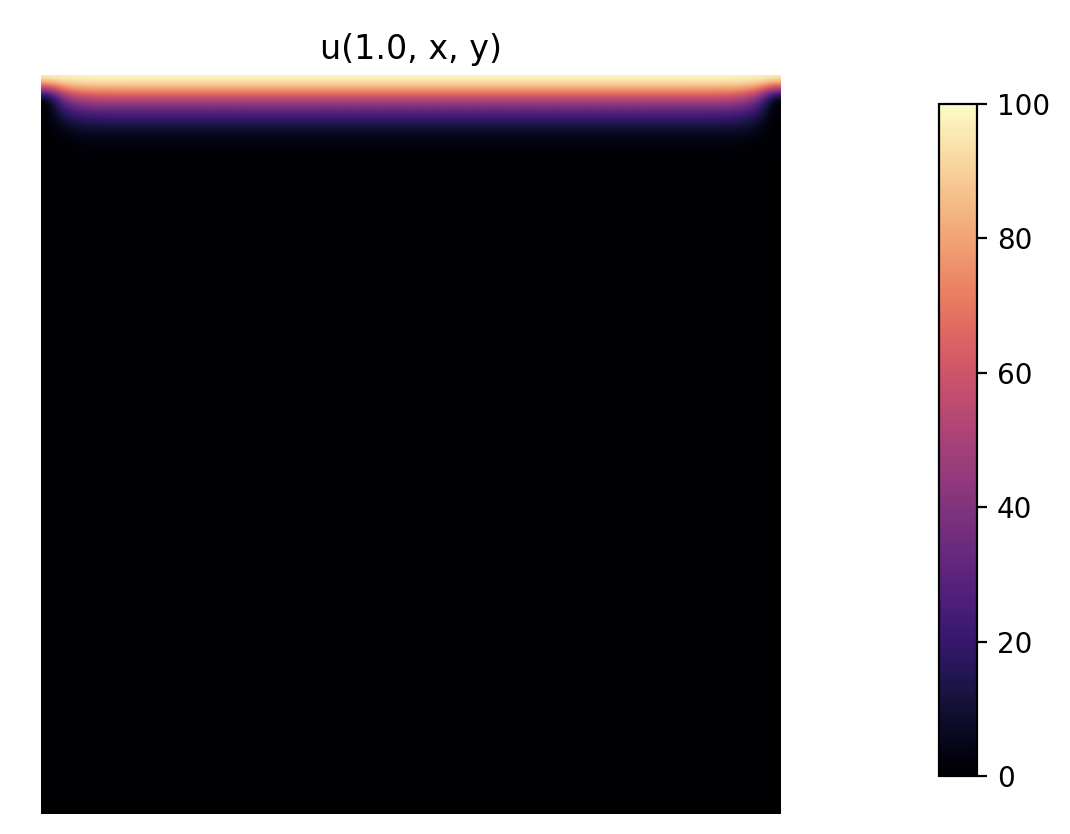
\includegraphics[width=0.95\linewidth]{img/1._diff.png} 
\end{minipage} 
\begin{minipage}[b]{0.50\linewidth}
	\centering
	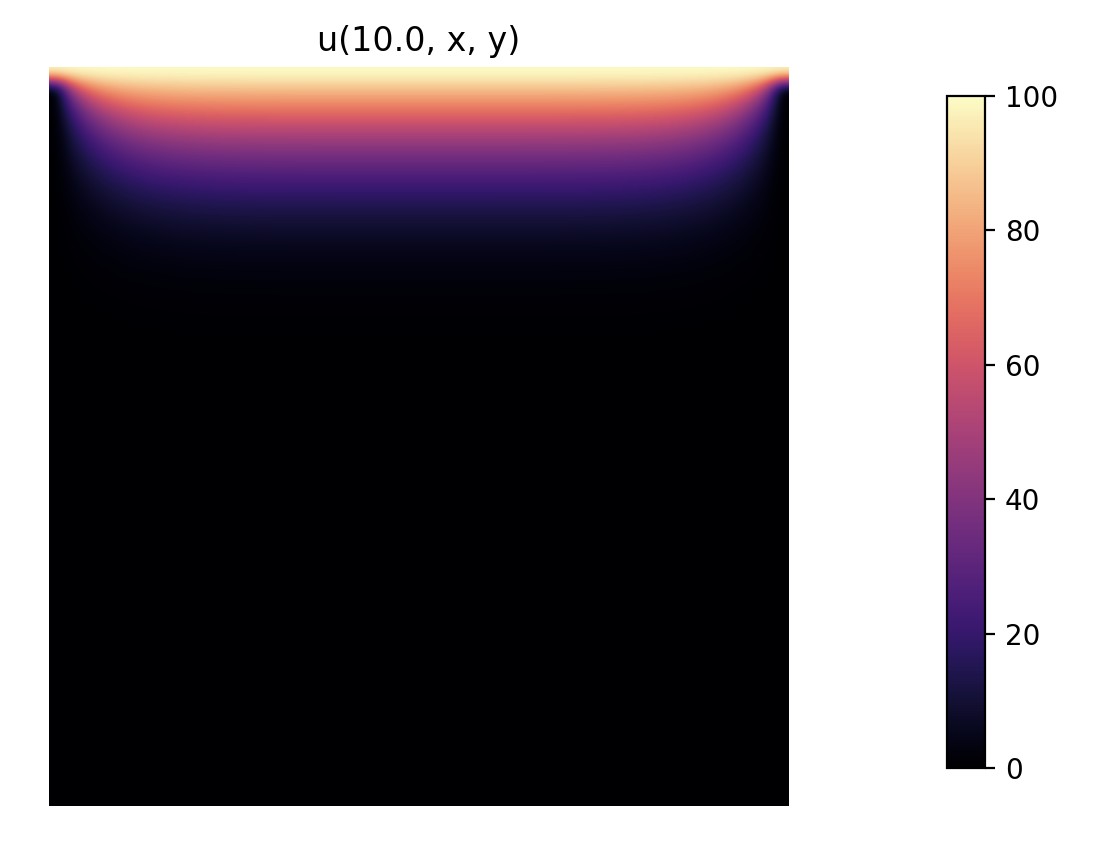
\includegraphics[width=0.95\linewidth]{img/10._diff.png} 
\end{minipage} 
\begin{minipage}[b]{0.50\linewidth}
	\centering
	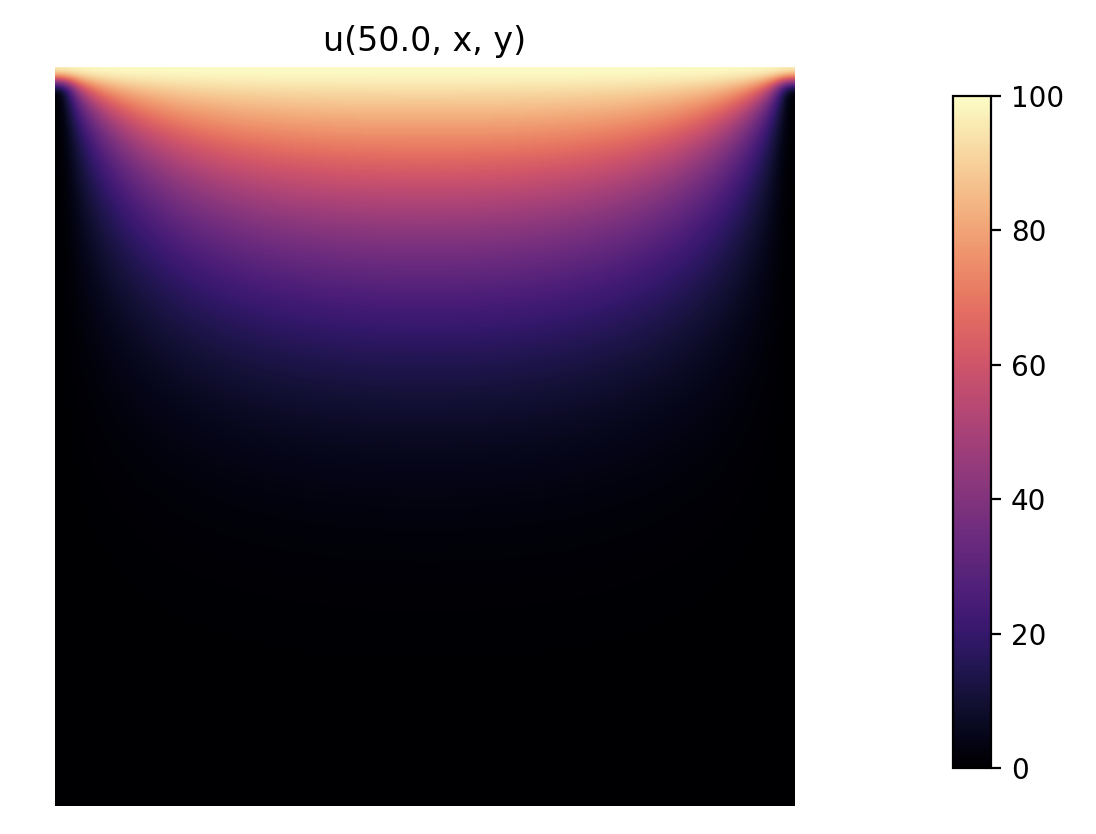
\includegraphics[width=0.95\linewidth]{img/50._diff.png}
\end{minipage}
\hfill 
\begin{minipage}[b]{0.50\linewidth}
	\centering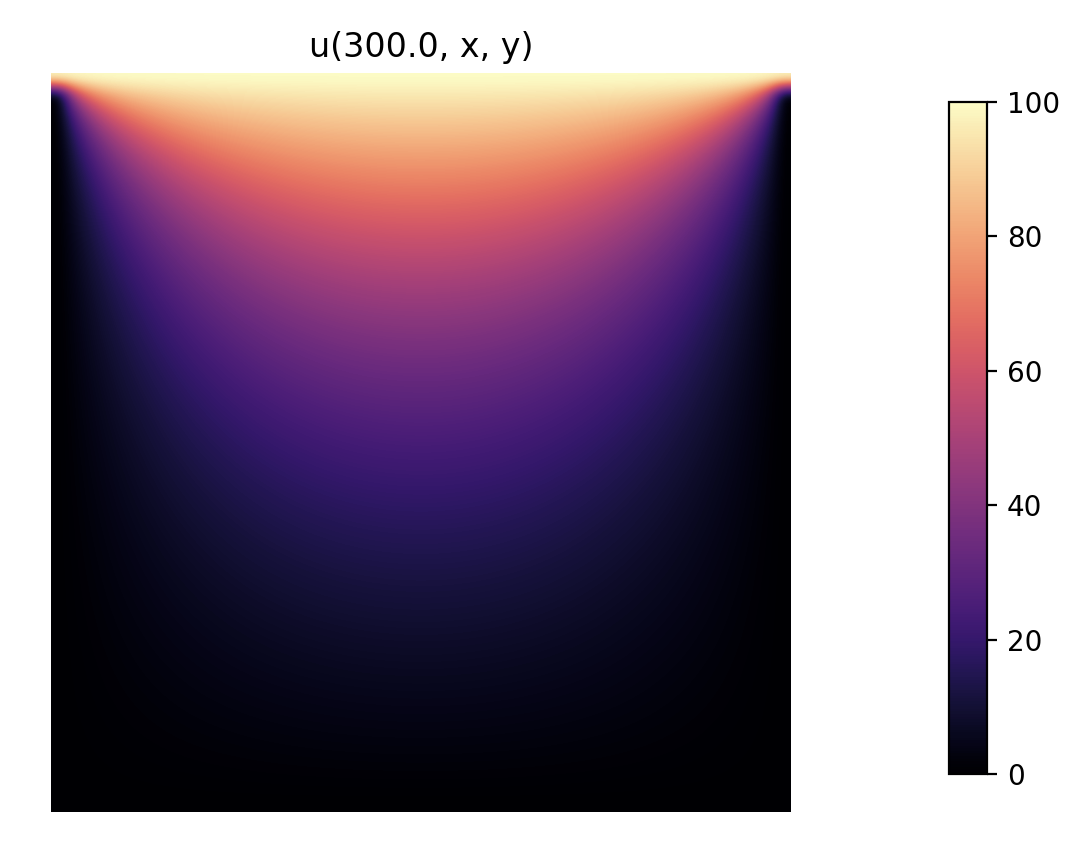
\includegraphics[width=0.95\linewidth]{img/300._diff.png} 
\end{minipage} 
\caption{Solution of $u(t, x, y)$ as described in Section~\ref{problem} for $(x, y) \in [0, 50] \times [0, 50]$, and for $t \in \{1, 10, 50, 300\}$.}
\label{sol} 
\end{figure}

\section{Convergence rate analysis}
\subsection{Method}
\label{methodSS}

We denote by $\Tilde{u}_k^{i, j}$ the solution of the implemented finite scheme at point $(t_k, x_i, y_j) := (kL_t/n_t, iL_x/n_x, jL_y/n_y) \in \Omega$. We define the following sequence: 
\begin{equation}
	e_k^{i, j} = \left| \Tilde{u}_k^{i, j} - u(t_k, x_i, y_j) \right|.
\end{equation}

We are looking for the rates of convergence of the scheme i.e., $r_t, r_x, r_y \in \mathbb{R}$ such that, for some constants $C_t, C_x$ and $C_y$:
\begin{equation}
\label{rate}
	\| \Tilde{u}(t, x, y) - u(t, x, y) \| \leq C_t \Delta_t^{r_t} + C_x \Delta_x^{r_x} + C_y \Delta_y^{r_y}, 
\end{equation}
where $\Tilde{u}$ is a defined by part approximation function from the sequence $\left( \tilde{u}_k^{i, j} \right)$.

In order to approximate the left hand side of \eqref{rate}, we will analyze the following errors, respectively approximations of norms $\| \cdot \|_1$, $\| \cdot \|_2$ and $\| \cdot \|_\infty$\footnote{For information, $E_2$ is chosen in the same fashion as in \cite{book} and $E_\infty$ in the same fashion as in \cite{morton_mayers_2005}.}:
\begin{equation}
	E_1(n_t, n_x, n_y) := \frac{\sum_{k = 0}^{n_t} \sum_{i = 0}^{n_x} \sum_{j = 0}^{n_y} e_k^{i, j}}{(n_t + 1) + (n_x + 1) + (n_y + 1)},  
\end{equation}
\begin{equation}
	E_2(n_t, n_x, n_y) := \left( \Delta t \Delta x \Delta y \sum_{k = 0}^{n_t} \sum_{i = 0}^{n_x} \sum_{j = 0}^{n_y} \left(e_k^{i, j}\right)^2 \right )^{1/2}, 
\end{equation}
\begin{equation}
	E_\infty(n_t, n_x, n_y)  := \max_{\substack{k \in \{ 0, \dots, n_t\} \\ i \in \{ 0, \dots, n_x\} \\ j \in \{ 0, \dots, n_y \} }} e_k^{i, j}.
\end{equation}

Suppose we want to find $r_x$. It holds that, for some error $E = E_1, E_2, E_\infty$, for $n_x$ large enough:
\begin{equation}
\label{method}
	\log_2\left( \frac{E(n_t, n_x, n_y)}{E(n_t, 2n_x, n_y)} \right) \approx \log_2\left(  \frac{C_x \Delta x^{r_x}}{C_x \left( \frac{\Delta x}{2} \right)^{r_x}} \right) = \log_2 \left( 2^{r_x} \right) = r_x.
\end{equation}

Thus, for different values of $n_x$ and for all the considered errors, we can compute the quantity written above and consider it as an approximation of $r_x$. We can apply the same method to find $r_t$ and $r_y$. 

The Euler explicit scheme (applied for $t$) has a rate of convergence of $1$, and the central difference (applied for $x$ and $y$) has a rate of convergence of $2$. We thus expect to find $r_t \approx 1$, $r_x \approx 2$ and $r_y \approx 2$ (see \cite[Section~3.6.6]{book}).

\subsection{Convergence rate w.r.t. $n_t$}

Since we do not know the analytical solution of PDE \eqref{PDE}, we choose large enough values of $n_t$, $n_x$ and $n_y$ compared to those used for the experiment. We consider in our computations that $\Tilde{u}_k^{i, j}$ with these values of $(n_t, n_x, n_y)$ is the analytical solution. For this experiment, we choose to take as reference $(n_t, n_x, n_y) = (76800, 50, 50)$. We will now compute the quantity expressed in \eqref{method} with $(n_x, n_y) = (50, 50)$, and $n_t \in \{ 2400, 4800, 9600, 19200 \}$\footnote{Note that, all along the report, values of $(n_t, n_x, n_y)$ are chosen such that condition~\eqref{stable} holds i.e., such that the numerical resolution is stable.}. Results of experiments to approximate $r_t$ are depicted in Table~\ref{tab:texp}.
\begin{table}[h!]
\centering
\begin{tabular}{lcccc}
\hline
$n_t$ & 2400 & 4800 & 9600 & 19200 \\ \hline
$E_1(n_t, 50, 50)$ & $5.470 \times 10^{-3}$ & $2.651 \times 10^{-3}$ & $1.238 \times 10^{-3}$ & $5.308 \times 10^{-4}$ \\
$E_2(n_t, 50, 50)$ & $6.621 \times 10^{1}$ & $3.146 \times 10^{1}$ & $1.457 \times 10^{1}$ & $6.225 \times 10^{0}$ \\
$E_\infty(n_t, 50, 50)$ & $1.947 \times 10^{1}$ & $1.054 \times 10^{1}$ & $5.221 \times 10^{0}$ & $2.307 \times 10^{0}$ \\ \hline
$ r_t \approx \log_2\left( \frac{E_1(n_t, n_x, n_y)}{E_1(2n_t, n_x, n_y)} \right) $ & 1.045 & 1.098 & 1.222 &  \\
$ r_t \approx \log_2\left( \frac{E_2(n_t, n_x, n_y)}{E_2(2n_t, n_x, n_y)} \right) $ & 1.074 & 1.110 & 1.227 &  \\
$ r_t \approx \log_2\left( \frac{E_\infty(n_t, n_x, n_y)}{E_\infty(2n_t, n_x, n_y)} \right) $ & 0.885 & 1.013 & 1.178 &  \\ \hline
\end{tabular}
\caption{Experiments to approximate $r_t$, for $n_t \in \{ 2400, 4800, 9600, 19200 \}$}
\label{tab:texp}
\end{table}

One can observe that, as expected, the value of $r_t \approx 1$ (c.f. Section~\ref{methodSS}) for all the considered errors.

\subsection{Convergence rate w.r.t. $n_x$}

In the same way as for the experiment above, we choose reference values for $(n_t, n_x, n_y)$ i.e., $(19200, 128, 128)$. We will now compute the quantity expressed in \eqref{method} with $(n_t, n_y) = (19200, 128)$, and $n_x \in \{ 8, 16, 32, 64 \}$. Results of experiments to approximate $r_x$ are depicted in Table~\ref{tab:xexp}.
\begin{table}[h!]
\centering
\begin{tabular}{lcccc}
\hline
$n_x$ & 8 & 16 & 32 & 64 \\ \hline
$E_1(19200, n_x, 128)$ & $2.293 \times 10^{-1}$ & $7.797 \times 10^{-1}$ & $2.312 \times 10^{-2}$ & $5.344 \times 10^{-3}$ \\
$E_2(19200, n_x, 128)$ & $4.851 \times 10^{2}$ & $2.235 \times 10^{2}$ & $9.860 \times 10^{1}$ & $3.381 \times 10^{1}$ \\
$E_\infty(19200, n_x, 128)$ & $6.578 \times 10^{0}$ & $6.532 \times 10^{0}$ & $6.347 \times 10^{0}$ & $5.521 \times 10^{0}$ \\ \hline
$ r_x \approx \log_2\left( \dfrac{E_1(n_t, n_x, n_y)}{E_1(n_t, 2n_x, n_y)} \right) $ & 1.556 & 1.754 & 2.113 &  \\
$ r_x \approx \log_2\left( \dfrac{E_2(n_t, n_x, n_y)}{E_2(n_t, 2n_x, n_y)} \right) $ & 1.118 & 1.181 & 1.544 &  \\
$ r_x \approx \log_2\left( \dfrac{E_\infty(n_t, n_x, n_y)}{E_\infty(n_t, 2n_x, n_y)} \right) $ & 0.010 & 0.041 & 0.201 &  \\ \hline
\end{tabular}
\caption{Experiments to approximate $r_x$, for $n_x \in \{ 8, 16, 32, 64 \}$}
\label{tab:xexp}
\end{table}

One can see that, by considering $E_1$, $r_x$ is approximately its expected value i.e., 2. When $E_2$ is considered, one can observe that the approximation of $r_x$ tends to grow and goes above 1.5. However, when $E_\infty$ is considered, the maximal value attained by the approximation of $r_x$ is no larger than $0.3$.

We interpret these results in the following way. First, a coarse mesh allows for a worse approximation of $r_x$. Second, a $p$-norm $\| \cdot \|_p$ is more and more sensitive to inaccuracy for larger and larger $p$. This allows us to conclude that $E_2$ would need finer meshes to attain $r_x \approx 2$, and it is even more the case for $E_\infty$.

However, for the approximation to be good, since the reference sequence $\left(\tilde{u}_k^{i, j}\right)$ needs to be very accurate in comparaison to those computed for the experience (i.e. with $n_x \in \{8, 16, 32, 64\}$), we would need to re-do the experiments with larger values of $n_x$. For computational reasons (in space and time), we cannot find stable values of $(n_t, n_x, n_y)$ for the reference and the computed solutions such that the approximation is good for both $E_2$ and $E_\infty$. For this reason we choose to restrict ourselves to $E_1$ for this experiment.

\subsection{Convergence rate w.r.t. $n_y$}

In order to approximate $r_y$, we do exactly the same as for $r_x$ (same reference) but by computing values of $\tilde{u}_k^{i, j}$ for $(n_t, n_x) = (19200, 128)$ and $n_y \in \{ 8, 16, 32, 64 \}$. Results of experiments to approximate $r_y$ are depicted in Table~\ref{tab:yexp}.
\begin{table}[h!]
\centering
\begin{tabular}{lcccc}
\hline
$n_y$ & 8 & 16 & 32 & 64 \\ \hline
$E_1(19200, 128, n_y)$ & $1.745 \times 10^{-1}$ & $6.138 \times 10^{-2}$ & $1.877 \times 10^{-2}$ & $4.432 \times 10^{-3}$ \\
$E_2(19200, 128, n_y)$ & $4.110 \times 10^{2}$ & $1.990 \times 10^{2}$ & $9.154 \times 10^{1}$ & $3.192 \times 10^{1}$ \\
$E_\infty(19200, 128, n_y)$ & $3.023 \times 10^{0}$ & $2.956 \times 10^{0}$ & $2.540 \times 10^{0}$ & $1.803 \times 10^{0}$ \\ \hline
$ r_y \approx \log_2\left( \frac{E_1(n_t, n_x, n_y)}{E_1(n_t, n_x, 2n_y)} \right) $ & 1.507 & 1.709 & 2.082 &  \\
$ r_y \approx \log_2\left( \frac{E_2(n_t, n_x, n_y)}{E_2(n_t, n_x, 2n_y)} \right) $ & 1.046 & 1.121 & 1.520 &  \\
$ r_y \approx \log_2\left( \frac{E_\infty(n_t, n_x, n_y)}{E_\infty(n_t, n_x, 2n_y)} \right) $ & 0.032 & 0.219 & 0.495 &  \\ \hline
\end{tabular}
\caption{Experiments to approximate $r_y$, for $n_y \in \{ 8, 16, 32, 64 \}$}
\label{tab:yexp}
\end{table}

By symmetry, we obtain very similar results as for $r_x$.

\bibliographystyle{plain}
\bibliography{ref}

\end{document}
